\documentclass[12pt,a4paper]{article}
\usepackage[left=15mm,right=15mm,top=14mm,bottom=20mm,footskip=10mm]{geometry}
\usepackage{iftex}
\ifPDFTeX
  \usepackage[T5]{fontenc}
  \usepackage[utf8]{inputenc}
  \usepackage{mathptmx}
\else
  \usepackage{fontspec}
  \setmainfont{Times New Roman}
\fi
\usepackage{amsmath,amssymb}
\usepackage{fix-cm}
\usepackage{tikz}
\usetikzlibrary{arrows.meta}
\usepackage{tcolorbox}
\usepackage{fancyhdr}
\usepackage{lastpage}
\usepackage{tabularx}
\definecolor{sectionpurple}{RGB}{155,42,143}
\definecolor{notebackground}{RGB}{229,240,245}
\definecolor{noteborder}{RGB}{255,55,55}
\setlength{\parindent}{0pt}
\setlength{\parskip}{2pt}
\setlength{\headheight}{15pt}
\pagestyle{fancy}
\fancyhf{}
\renewcommand{\headrulewidth}{0pt}
\renewcommand{\footrulewidth}{0.4pt}
\fancyfoot[L]{\fontsize{8.5}{10}\selectfont
  Biên soạn: \textbf{Nguyễn Anh Dũng}}
\fancyfoot[R]{\fontsize{8.5}{10}\selectfont
  Trang \thepage/\pageref{LastPage} -- Đề TDMXX01B}

\newtcolorbox{notebox}{colback=notebackground,colframe=noteborder,
  boxrule=0.8pt,arc=2pt,left=8pt,right=8pt,top=4pt,bottom=4pt,
  before skip=4pt,after skip=4pt}

\newcommand{\question}[2][TDM21]{%
  \par\addvspace{5pt}\noindent
  \textbf{\textcolor{sectionpurple}{Câu #2:} \textcolor{noteborder}{[#1]}}\enspace
}
\newcommand{\answerlabel}[1]{\textbf{\textcolor{sectionpurple}{#1.}}}
\newcommand{\fourchoices}[4]{%
  \par\nobreak\smallskip
  \begin{tabular*}{\linewidth}{@{}l@{\extracolsep{\fill}}lll@{}}
    \answerlabel{A} #1 & \answerlabel{B} #2 & \answerlabel{C} #3 & \answerlabel{D} #4
  \end{tabular*}\par
}
\newcommand{\twochoices}[4]{%
  \par\nobreak\smallskip
  \begin{tabularx}{\linewidth}{@{}>{\raggedright\arraybackslash}X>{\raggedright\arraybackslash}X@{}}
    \answerlabel{A} #1 & \answerlabel{B} #2 \\[2pt]
    \answerlabel{C} #3 & \answerlabel{D} #4
  \end{tabularx}\par
}
\newcommand{\shortanswer}{%
  \par\nobreak\hfill
  
\begin{tikzpicture}
    \node[draw=noteborder,fill=notebackground,line width=0.8pt,
      rounded corners=2pt,minimum width=24mm,minimum height=6mm,inner sep=0pt] {};
  \end{tikzpicture}\par
}

\newcommand{\extremagraph}{%
\begin{notebox}
\centering
\begin{tikzpicture}[x=0.62cm,y=0.40cm,
  every node/.style={font=\fontsize{11.5}{14}\selectfont}]
  \draw[thin,-{Stealth[length=4pt]}] (-6.2,0) -- (8.2,0) node[below] {$x$};
  \draw[thin,-{Stealth[length=4pt]}] (0,-5) -- (0,8.8) node[left] {$y$};
  \draw[thin,densely dashed] (-2,0) -- (-2,6);
  \draw[thin,densely dashed] (0,6) -- (-2,6);
  \draw[thin,densely dashed] (5,0) -- (5,-3);
  \draw[thin,densely dashed] (0,-3) -- (5,-3);
  \draw[sectionpurple,thick]
    (-5.1,-1.1) .. controls (-4.2,2.7) and (-3.2,6.0) .. (-2,6)
    .. controls (-0.8,6.0) and (2.7,-3) .. (5,-3)
    .. controls (6.0,-3) and (6.9,1.8) .. (7.7,6.7);
  \fill (-2,6) circle (1.4pt);
  \fill (5,-3) circle (1.4pt);
  \fill (-2,0) circle (1.2pt);
  \fill (5,0) circle (1.2pt);
  \node[below left] at (0,0) {$O$};
  \node[below] at (-2,0) {$-2$};
  \node[above] at (5,0) {$5$};
  \node[right] at (0,6) {$6$};
  \node[left] at (0,-3) {$-3$};
  \node[right,sectionpurple] at (7.1,5.9) {$f(x)$};
\end{tikzpicture}
\end{notebox}
}

\newcommand{\tfbox}[4]{%
\begin{notebox}
\renewcommand{\arraystretch}{1.45}
\setlength{\tabcolsep}{5pt}
\begin{tabularx}{\linewidth}{|>{\bfseries\color{sectionpurple}}c|>{\raggedright\arraybackslash}X|c|c|}
\hline
\multicolumn{2}{|c|}{\textbf{\textcolor{sectionpurple}{Mệnh đề}}}
& \textbf{\textcolor{sectionpurple}{Đ}} & \textbf{\textcolor{sectionpurple}{S}} \\
\hline
a & #1 & $\bigcirc$ & $\bigcirc$ \\[2pt]\hline
b & #2 & $\bigcirc$ & $\bigcirc$ \\[2pt]\hline
c & #3 & $\bigcirc$ & $\bigcirc$ \\[2pt]\hline
d & #4 & $\bigcirc$ & $\bigcirc$ \\[2pt]\hline
\end{tabularx}
\end{notebox}
}

\begin{document}
\fontsize{12}{15}\selectfont

{\centering
\textbf{ĐỀ TDMXX01B}\par
\textbf{CỰC TRỊ CỦA HÀM SỐ}\par
{\fontsize{10.5}{13}\selectfont\itshape
Form đề chuẩn bám sát BGD2025 -- Thời gian làm bài \textbf{90 phút}\par}}

\textbf{Phần I. Câu trắc nghiệm nhiều phương án lựa chọn.}
Thí sinh trả lời từ câu 1 đến câu 12. Mỗi câu hỏi thí sinh chỉ chọn một phương án.

\question{1} Điểm cực đại của hàm số $y=x^3-3x+3$ là:
\fourchoices{$x=-1$}{$x=1$}{$y=5$}{$y=1$}

\question{2} Cho hàm số $y=3x^3-3x^2+1$. Điểm cực tiểu của hàm số tương ứng là:
\fourchoices{$x=0$}{$y=1$}{$x=2$}{$y=-3$}

\question{3} Trong các hàm số dưới đây, hàm số nào có nhiều điểm cực trị nhất?
\fourchoices{$y=x^3-3x$}{$y=x^4+x^2-2021$}
{$y=\dfrac{2x-1}{x+1}$}{$y=2x-\sin x$}

\question{4} Trong các hàm số dưới đây, hàm số nào có nhiều điểm cực trị nhất?
\twochoices{$y=x^3-2x^2$}{$y=x^4-3x^2+1$}
{$y=x^{2021}-3x^{100}-x$}{$y=2021+\cos 2x$}

\question{5} Cho hàm số $y=f(x)$ có đồ thị như hình vẽ bên dưới. Mệnh đề đúng là:
\extremagraph
\twochoices{Điểm cực tiểu của hàm số là $y=-3$.}
{Giá trị cực đại của hàm số là $x=6$.}
{Giá trị cực tiểu của hàm số là $y=-3$.}
{Điểm cực đại của hàm số là $x=5$.}

\question{6} Cho hàm số $y=f(x)$ có đồ thị như hình vẽ bên dưới. Mệnh đề đúng là:
\extremagraph
\twochoices{Điểm cực tiểu của đồ thị hàm số $y=f(x)$ là $x=5$.}
{Điểm cực đại của đồ thị hàm số $y=f(x)$ là $(-2;6)$.}
{Điểm cực tiểu của đồ thị hàm số $y=f(x)$ là $(-3;5)$.}
{Điểm cực tiểu của đồ thị hàm số $y=f(x)$ là $y=-3$.}

\question{7} Hàm số $y=\sin x$ có tất cả bao nhiêu điểm cực trị trên $\mathbb{R}$?
\fourchoices{$1$}{$0$}{$2$}{Vô số}

\question{8} Hàm số $y=x^4-8x^2-1$ có tất cả bao nhiêu điểm cực tiểu?
\fourchoices{$2$}{$1$}{$3$}{$0$}

\question{9} Hàm số $y=x^4+2021x^2$ có tất cả bao nhiêu điểm cực tiểu?
\fourchoices{$3$}{$2$}{$0$}{$1$}

\question{10} So với hàm số $y=f(x)=x^4-4x^2$ thì hàm số $y=g(x)=-x^4-x^2$ có:
\twochoices{nhiều điểm cực đại hơn.}{nhiều điểm cực tiểu hơn.}
{bằng số điểm cực đại.}{bằng số điểm cực tiểu.}

\question{11} Cho các hàm số
\[
y=x^5+x+1;\quad y=x^3+3x;\quad y=-x^3+x;\quad
y=x^4-x^2;\quad y=x^4+x^2;\quad y=\frac{ax+b}{cx+d}.
\]
Hỏi có tất cả bao nhiêu hàm số không có cực trị?
\fourchoices{$1$}{$2$}{$4$}{$3$}

\question{12} Cho hàm số $y=f(x)$ có đồ thị như hình vẽ. Hàm số $f(x)$ có
\begin{notebox}
\centering
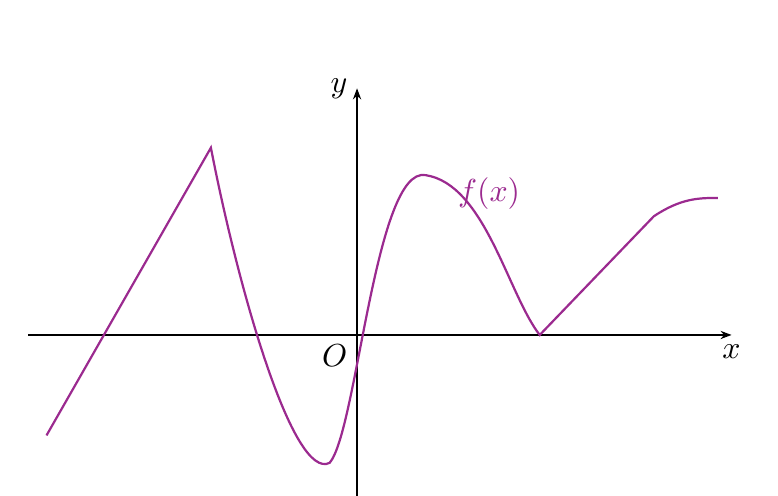
\begin{tikzpicture}[x=0.58cm,y=0.58cm,
  every node/.style={font=\fontsize{11.5}{14}\selectfont}]
  \draw[thin,-{Stealth[length=4pt]}] (-7.2,0) -- (8.2,0) node[below] {$x$};
  \draw[thin,-{Stealth[length=4pt]}] (0,-3.8) -- (0,5.4) node[left] {$y$};
  \draw[sectionpurple,thick]
    (-6.8,-2.2) -- (-3.2,4.1)
    .. controls (-2.6,1.0) and (-1.4,-3.2) .. (-0.6,-2.8)
    .. controls (0.0,-2.1) and (0.4,3.7) .. (1.5,3.5)
    .. controls (2.8,3.3) and (3.3,0.9) .. (4.0,0)
    -- (6.5,2.6)
    .. controls (7.1,3.0) and (7.5,3.0) .. (7.9,3.0);
  \node[below left] at (0,0) {$O$};
  \node[right,sectionpurple] at (2.0,3.1) {$f(x)$};
\end{tikzpicture}
\end{notebox}
\twochoices{tất cả là $5$ điểm cực trị.}{tất cả là $2$ điểm cực tiểu.}
{tất cả là $3$ điểm cực đại.}{tất cả là $2$ điểm cực trị.}

\par\addvspace{7pt}
\textbf{Phần II. Câu trắc nghiệm đúng sai.}
Thí sinh trả lời từ câu 13 đến câu 16. Trong mỗi ý \textbf{a), b), c), d)} ở mỗi câu,
thí sinh chọn \textbf{đúng} hoặc \textbf{sai}.

\question[TDM21]{13} Cho hàm số $y=f(x)$ có đạo hàm $f'(x)$ liên tục trên $\mathbb{R}$.
Hỏi trong các mệnh đề dưới đây, mệnh đề nào \textbf{đúng}, mệnh đề nào \textbf{sai}?
\tfbox
{Nếu $f'(x_0)=0$ thì hàm số $f(x)$ đạt cực trị tại điểm $x_0$.}
{Nếu $f'(x_0)=0$ và $f'(x)$ đổi dấu khi đi qua $x_0$ thì hàm số đạt cực trị tại điểm $x_0$.}
{Nếu $f'(x_0)=0$ và $f'(x)$ đổi dấu từ dương sang âm khi đi qua $x_0$ thì $x_0$ là điểm cực tiểu của hàm số $f(x)$.}
{Nếu $f'(x_0)=0$ và $f'(x)$ đổi dấu từ âm sang dương khi đi qua $x_0$ thì $x_0$ là điểm cực tiểu của đồ thị hàm số $y=f(x)$.}

\question[TDM32]{14} Cho hàm số $y=f(x)=x^4-2x^2+3$ có đồ thị $(C)$.
Biết rằng $(C)$ có ba điểm cực trị $A,B,C$ với điểm $A$ nằm trên trục tung và điểm $B$ nằm bên phải trục tung.
Hỏi trong các mệnh đề dưới đây, mệnh đề nào \textbf{đúng}, mệnh đề nào \textbf{sai}?
\tfbox
{$A(0;3)$.}
{$B(1;2)$.}
{Tam giác $ABC$ cân tại $A$.}
{Bán kính đường tròn ngoại tiếp tam giác $ABC$ bằng $1$.}

\question[TDM32]{15} Cho hàm số $y=f(x)$ có
\[
f'(x)=x(x-1)(x-3)^2(x-a),\qquad \forall x\in\mathbb{R},
\]
với $a$ là một số thực. Hỏi trong các mệnh đề dưới đây, mệnh đề nào \textbf{đúng}, mệnh đề nào \textbf{sai}?
\tfbox
{Khi $a=0$ thì hàm số có đúng một điểm cực trị.}
{Có đúng hai giá trị thực của $a$ để hàm số có đúng một điểm cực trị.}
{Hàm số có ba điểm cực trị khi và chỉ khi $a\in\{0;1;3\}$.}
{Hàm số $f(x)$ chỉ có tối đa $3$ điểm cực trị với mọi giá trị thực của $a$.}

\question[TDM32]{16} Cho hàm số $y=f(x)$ là hàm đa thức bậc bốn có đồ thị $(C)$.
Biết đồ thị $(C)$ có hai điểm cực trị liên tiếp nhau với tọa độ là $A(0;2),B(3;5)$,
hàm số $f(x)$ đạt cực trị tại $x=4$.
Hỏi trong các mệnh đề dưới đây, mệnh đề nào \textbf{đúng}, mệnh đề nào \textbf{sai}?
\tfbox
{Hàm số $f(x)$ đồng biến trên khoảng $(0;3)$.}
{Hàm số $f(x)$ nghịch biến trên khoảng $(3;4)$.}
{Một giá trị cực tiểu của hàm số $f(x)$ là $-2$.}
{Ba điểm cực trị của $(C)$ tạo thành một tam giác vuông.}

\par\addvspace{7pt}
\textbf{Phần III. Câu trắc nghiệm trả lời ngắn.}
Thí sinh trả lời từ câu 17 đến câu 22.

\question[TDM32]{17} Cho hàm số $y=f(x)$ liên tục trên $\mathbb{R}$ và có biểu thức đạo hàm là
\[
f'(x)=\frac{x(x+1)}{\sqrt[3]{x-1}}.
\]
Hỏi hàm số $y=f(x)$ có tất cả bao nhiêu điểm cực trị?
\shortanswer

\question[TDM31]{18} Cho hàm số $y=f(x)$ liên tục trên $\mathbb{R}$ và có đồ thị đạo hàm
$y=f'(x)$ như hình vẽ bên dưới. Hỏi hàm số $y=2026f(x)+2027$ có bao nhiêu điểm cực trị?
\begin{notebox}
\centering
\begin{tikzpicture}[x=0.62cm,y=0.62cm,
  every node/.style={font=\fontsize{11.5}{14}\selectfont}]
  \draw[thin,-{Stealth[length=4pt]}] (-6.8,0) -- (7.2,0) node[below] {$x$};
  \draw[thin,-{Stealth[length=4pt]}] (0,-4.0) -- (0,5.3) node[left] {$y$};
  \draw[thin,densely dashed] (-2.2,-3.4) -- (-2.2,5.0);
  \draw[noteborder,thick]
    (-6.2,-3.0) .. controls (-4.4,-1.9) and (-3.1,-0.8) .. (-2.65,0)
    .. controls (-2.42,1.4) and (-2.30,3.6) .. (-2.25,5.0);
  \draw[noteborder,thick]
    (-2.05,-3.7) .. controls (-1.8,1.1) and (-1.2,4.3) .. (-0.4,4.4)
    .. controls (1.2,4.3) and (2.3,0.0) .. (3.6,0)
    .. controls (4.8,0) and (5.5,2.3) .. (6.2,5.0);
  \node[below left] at (0,0) {$O$};
  \node[right,noteborder] at (5.8,4.0) {$f'(x)$};
\end{tikzpicture}
\end{notebox}
\shortanswer

\question[TDM31]{19} Cho hàm số $f(x)=ax^3+bx^2+cx+d$ xác định trên $\mathbb{R}$ và có đồ thị $(C)$.
Biết đồ thị hàm số có hai điểm cực trị là $(0;2)$ và $(2;0)$.
Giá trị của biểu thức $(a+b+c+d)$ tương ứng bằng:
\shortanswer

\question[TDM32]{20} Cho hàm số $y=f(x)$ xác định trên $\mathbb{R}$, có các đồ thị
$y=f(x)$ trên $[0;+\infty)$ và đồ thị đạo hàm $y=f'(x)$ trên $(-\infty;0)$ như hình vẽ.
Hàm số $y=f(x)$ có bao nhiêu điểm cực trị?
\begin{notebox}
\centering
\begin{tikzpicture}[x=0.68cm,y=0.62cm,
  every node/.style={font=\fontsize{11.5}{14}\selectfont}]
  \draw[thin,-{Stealth[length=4pt]}] (-5.5,0) -- (6.0,0) node[below] {$x$};
  \draw[thin,-{Stealth[length=4pt]}] (0,-3.5) -- (0,5.2) node[left] {$y$};
  \draw[black,thick] (-4.9,-2.3) -- (0,3.1);
  \node[left] at (-3.0,1.0) {$f'(x)$};
  \draw[black,thick]
    (0,3.1) .. controls (0.7,5.0) and (1.4,4.6) .. (1.9,3.0)
    .. controls (2.7,0.0) and (3.0,-2.5) .. (3.8,-2.6)
    .. controls (4.6,-2.5) and (5.0,0.2) .. (5.5,1.5);
  \node[right] at (4.8,1.5) {$f(x)$};
  \node[below left] at (0,0) {$O$};
\end{tikzpicture}
\end{notebox}
\shortanswer

\question[TDM32]{21} Cho hàm số $y=f(x)$ có đạo hàm liên tục và xác định trên $\mathbb{R}$,
và có biểu thức đạo hàm là
\[
f'(x)=x(x-1)(x-3)\left(x^2-2mx+m+1\right).
\]
Hỏi có tất cả bao nhiêu giá trị nguyên của tham số $m\in[-20;20]$ để hàm số $y=f(x)$ đúng $5$ điểm cực trị?
\shortanswer

\question[TDM32]{22} Gieo một con súc sắc cân đối đồng chất ba lần liên tiếp.
Từ các số chấm thu được ở mỗi lần ta dựng một hàm số bậc ba có nhận các số chấm này là nghiệm
và gọi hàm bậc ba này là đạo hàm của hàm số $y=f(x)$.
Hãy tính xác suất để thu được một hàm số $f(x)$ có đúng ba điểm cực trị
(làm tròn kết quả đến hàng phần trăm)?
\shortanswer

\par\medskip
{\centering\textbf{\textcolor{sectionpurple}{--- Hết ---}}\par}

\end{document}
